\documentclass[a4paper,11pt,fleqn]{article}%fleqn pour aligner les equations à gauche
\usepackage{../../Styles/Eval}

\newcommand{\chnum}{DS5}
\newcommand{\chtitle}{DS 5 : Ondes et Cinétique chimique}
\newcommand{\dtype}{DS}

\begin{document}
	\maketitle
\section*{Exercice 1 : Décomposition de l'acide nitreux}
En solution aqueuse, l'acide nitreux \ce{HNO2} est peu stable et se transforme lentement en acide nitrique (\ce{H+(aq)},\ce{NO3-(aq)}) avec un dégagement de monoxyde d'azote \ce{NO}.\\
L'équation de la réaction est
\begin{eqnarray}
	\ce{2HNO2(aq) -> NO(g) + 2H+(aq) + NO3-(aq)} \nonumber
\end{eqnarray}
On suit l'évolution des concentrations [\ce{HNO2}] et [\ce{NO3-}] au cours du temps dans \num{100} \unit{\milli\liter} de solution d'acide nitreux de concentration initiale $c_0$ = \num{0,625} \unit{\mole\per\liter}.\\
\begin{center}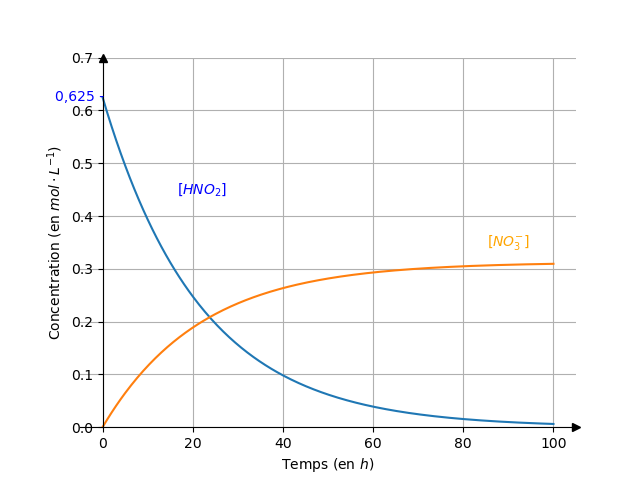
\includegraphics[scale=1]{Ressources/TSPE_C10_Eval_Fig5.png}\end{center}


\begin{enumerate}
	\item Construire un tableau d'avancement de la réaction
	\item Définir et calculer les vitesses volumiques de disparition de \ce{HNO2} et d'apparition de \ce{NO3-} à $t=0$.
	\item Expliquer une méthodologie, applicable ici, pour montrer que [\ce{HNO2}](t) suit une loi de vitesse d'ordre 1.
	\item Déterminer la date $t_1$ à laquelle les deux courbes se coupent. Quelle est la composition du mélange à cette date ?
	\item Déterminer la vitesses volumiques de disparition de \ce{HNO2} et d'apparition de \ce{NO3-} à la date $t_1$.
	\item Déterminer le temps de demi-réaction $t_{1/2}$.
\end{enumerate}

\section*{Exercice 2 : Étude d'un écran de smartphone}
Lorsqu'il est allumé, un écran de téléphone portable est constitué de pixels (contraction de \emph{picture elements}) en forme de petits carrés de luminosité et de couleurs différentes qui forment l'image affichée. Chaque pixel est composé lui-même d'un ensemble de trois luminophores de  couleurs respectives rouge, vert et bleu.

\subsection{Diffraction par un petit miroir}

\begin{minipage}{.45\linewidth}
	Lorsqu'un faisceau laser se réfléchit sur un  très petit miroir rectangulaire de grande hauteur et de largeur très petite, monté sur un support, on observe sur un écran une figure de diffraction analogue à celle observée lorsque ce faisceau laser traverse une fente dont les dimensions sont les mêmes que celles du miroir.\\
	On note $a$ la largeur du miroir, $D$ la distance entre le miroir et l'écran et $\lambda$ la longueur d'onde du laser utilisé.\\
	On note $\theta$ l'écart angulaire (exprimé en radians) entre le milieu de la tache centrale brillante et la première extinction.
\end{minipage}
\begin{minipage}{.45\linewidth}
	\centering
	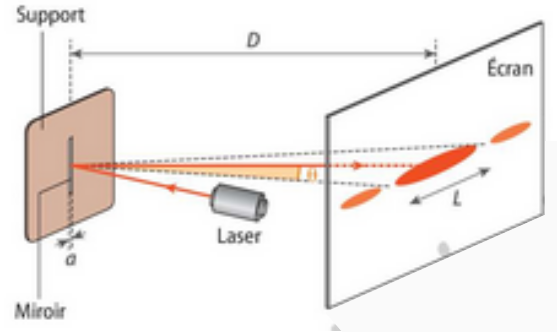
\includegraphics[scale=.6]{Ressources/TSPE_C10_Eval_Fig4.png}
\end{minipage}
	
	\begin{enumerate}
		\item 
			\begin{enumerate}
				\item Donner, en le justifiant, un ordre de grandeur possible de la largeur $a$ du miroir, si on utilise une lumière visible pour observer une figure de diffraction.
				\item Rappeler la relation entre l'écart angulaire $\theta$, la largeur du miroir $a$ et la longueur d'onde $\lambda$.
				\item Voici les deux figures de diffraction par réflexion obtenues sur un écran avec un laser vert (Figure 1) puis avec un laser rouge (Figure 2).\\
				Sachant que le laser rouge utilisé a une longueur d'onde $\lambda_R$ = \num{632,8} \unit{\nano\meter}, déterminer celle du laser vert notée $\lambda_V$.
			\end{enumerate}
	\end{enumerate}
\begin{figure}[h!]
	\centering
	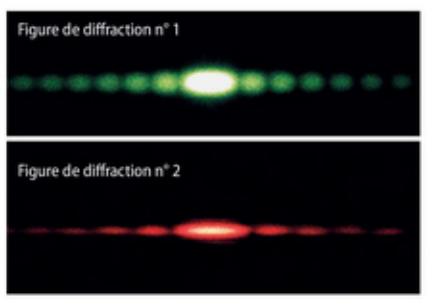
\includegraphics[scale=.9]{Ressources/TSPE_C10_Eval_Fig2.png}
\end{figure}
	
	\subsection{Détermination de la taille d'un pixel}
	\begin{minipage}{.45\linewidth}
		On braque maintenant le laser rouge vers l'écran d'un smartphone. Les pixels sont assimilés à une juxtaposition de très petits miroirs carrés accolés de coté $b$. Le dispositif expérimental est schématisé sur la figure suivante.\\
		On observe la figure obtenue sur un écran quadrillé.\\
		Cette figure est assimilable à une figure d'interférences à deux dimensions : l'interfrange $i$, distance entre deux points lumineux consécutifs sur l'axe horizontal ou sur l'axe vertical, est lié à la distance $b$ entre les centres de deux miroirs sur l'on ou l'autre de ces axes et à la longueur d'onde $\lambda$ : $i=\dfrac{\lambda D}{b}$.		
	\end{minipage}
	\begin{minipage}{.45\linewidth}
		\centering
		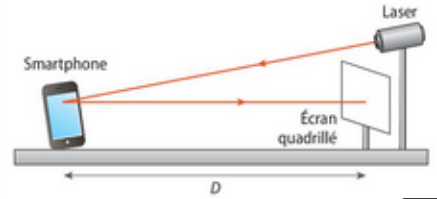
\includegraphics[scale=.6]{Ressources/TSPE_C10_Eval_Fig3.png}
	\end{minipage}

	\textbf{Données :}
	\begin{itemize*}
		\item Distance entre l'écran du smartphone et l'écran quadrillé : $D$ = (\num{1,74} $\pm$ \num{0,03}) \unit{\meter}
		\item Longueur d'onde du laser : $\lambda$ = \num{632,8} \unit{\nano\meter}
	\end{itemize*}
	\begin{enumerate}
		\setcounter{enumi}{1}
		\item 
			\begin{enumerate}
				\item Déterminer le plus précisément possible la distance $i$ entre deux points lumineux consécutifs.
				\item En déduire la valeur du coté $b$ d'un pixel carré.
				\item Un écran de smartphone a une largeur de \num{6} \unit{\centi\meter} et une hauteur de \num{11} \unit{\centi\meter}.\\
				Estimer le nombre de pixels qu'il comporte.
			\end{enumerate}
	\end{enumerate}
\begin{figure}[h!]
	\centering
	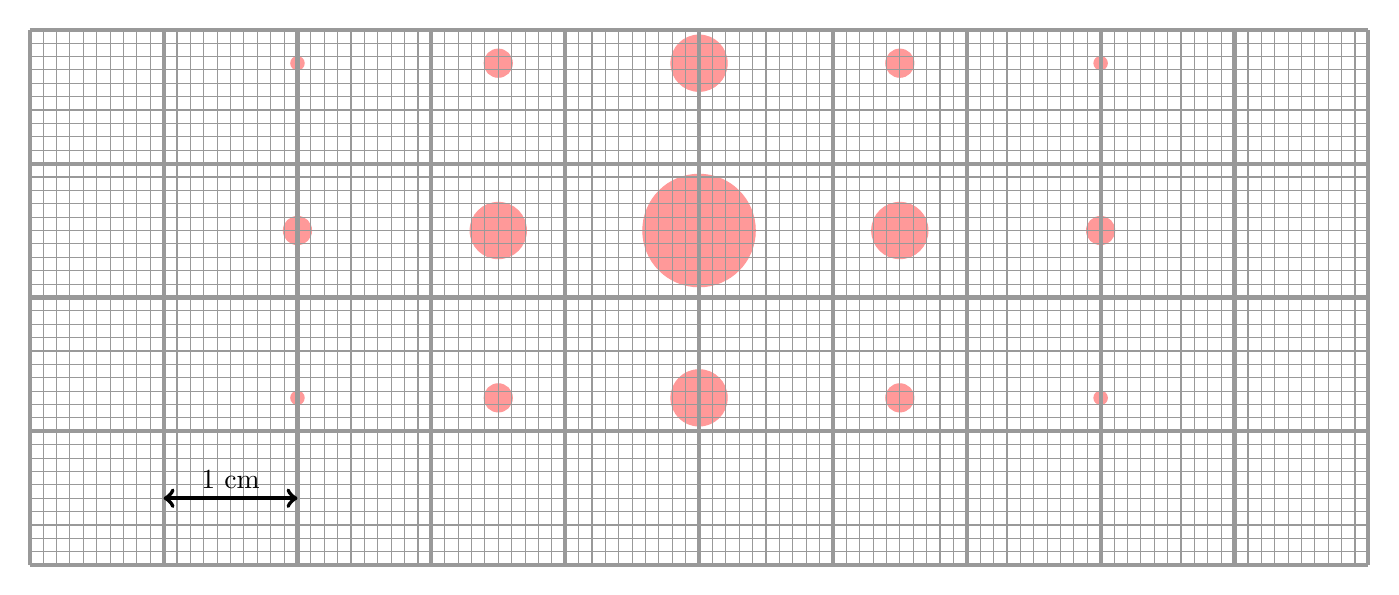
\begin{tikzpicture}[scale = 1.7]%figure d'interférence
		
		\filldraw[red!40] (5,2.5) circle (.42);
		\filldraw[red!40] (5,3.75) circle (.21);
		\filldraw[red!40] (5,1.25) circle (.21);
		\filldraw[red!40] (3.5,2.5) circle (.21);
		\filldraw[red!40] (6.5,2.5) circle (.21);
		
		
		\filldraw[red!40] (8,2.5) circle (.105);
		\filldraw[red!40] (2,2.5) circle (.105);
		\filldraw[red!40] (3.5,3.75) circle (.105);
		\filldraw[red!40] (6.5,3.75) circle (.105);
		\filldraw[red!40] (3.5,1.25) circle (.105);
		\filldraw[red!40] (6.5,1.25) circle (.105);
		
		\filldraw[red!40] (2,1.25) circle (.05);
		\filldraw[red!40] (2,3.75) circle (.05);
		\filldraw[red!40] (8,1.25) circle (.05);
		\filldraw[red!40] (8,3.75) circle (.05);
		
		\foreach \k in {0,0.1,...,4} {
			\draw[gray!80] (0,\k) -- (10,\k);}
		\foreach \k in {0,0.1,...,10} {
			\draw[gray!80] (\k,0) --(\k,4) ;}
		\foreach \k in {0,1,...,4} {
			\draw[gray!80,line width = 1.5] (0,\k) -- (10,\k);}
		\foreach \k in {0,1,...,10} {
			\draw[gray!80,line width = 1.5] (\k,0) --(\k,4) ;}
		\draw [<->, line width = 1.5] (1,.5) to (2,.5);
		\draw (1.5,.5) node[above]{1 cm};
	\end{tikzpicture}
\end{figure}
\end{document}